% 4  Results
% 4.1  Various plots with differing initial waves and bays ? including top-down view
% 4.1.1  Plots of same initial wave through different bays
% 4.1.1.1  Discuss resonance in terms of max. run up vs. max run up in plane-shaped bay (very large m)
% 4.1.1.1.1  Also in terms of how far up shore wave travels (top-down view)
% 4.1.2  Include at least one plot of eigenfunctions in both physical and sigma space
% 4.1.3  Include error in x wall mentioned previously in all different plots
% 4.2  Comparison to Pelinovsky?s analytic solution for m=2 and initial profile from paper
% 4.2.1  Comparison to initial condition
% 4.2.2  Alter number of eigenvalues, sigma (or x) steps, and lambda steps (each separately) to see what it takes to converge to analytic solution.
% 4.3  Possibly use max. run up and min. run down as a convergence metric - when varying number of eigenvalues, sigma (or x) steps, and lambda steps - for other values of m
% 4.4  Show how closely nonlinear system follows superposition principle ? measure of how linear/nonlinear the system is

\section{Results}

	\begin{frame}%Explain the problem with the standard forumula for relative error. 
		\frametitle{Error in Numerical Approximation}
		
		Relative Error $= |\frac{\text{Real Value } -\text{ Approximate Value}}{\text{Real Value}}|$\\\vspace{5mm}
		This implies \\\vspace{5mm}
		$|\text{Real Value } - \text{ Approximate Value}|=\text{Relative Error }  |\text{Real Value}|$
	
	\end{frame}



	\begin{frame}
		\frametitle{Error in Numerical Approximation Cont.}
		
		We modeled the N-wave where $A=.5, p=1.5, $ and $ \sigma_0=15$:\\\vspace{5mm}
		Max run up for N-wave is $\frac{8A}{3p^2}e^{-\frac{3}{2}}\approx0.1322$\\\vspace{5mm}
		Min run down for N-wave is $-\frac{4A}{3p^2}\
		\approx-0.29629$\\\vspace{5mm}
		\begin{center}
		\begin{tabular}{|c|c|c|c|}\hline
		$\Delta\lambda/\Delta\sigma$&$10^{-3}$&$10^{-4}$&$10^{-5}$\\\hline
		1&\specialcell{.0886\\-.1900}&NA&NA\\\hline
		$10^{-1}$&\specialcell{.1313\\-.2950}&\specialcell{.1313\\-.2950}&\specialcell{.1313\\-.2941}\\\hline
		$10^{-2}$&\specialcell{\textbf{.1319}\\\textbf{-.2963}}&\specialcell{.1319\\-.2963}&\specialcell{.1319\\-.2951}\\\hline
		\end{tabular}
		\end{center}
	\end{frame}

	\begin{frame}
	\frametitle{Error in Numerical Approximation Cont.}
	
	Relative error at min run-down: $.0026$\\\vspace{5mm}
	Relative error at max run-up : $.0091$\\\vspace{5mm}
	
	\end{frame}

	\begin{frame}
		\frametitle{Parabolic Case with Error Comparison}
		\begin{center}
		\includemovie[poster,text={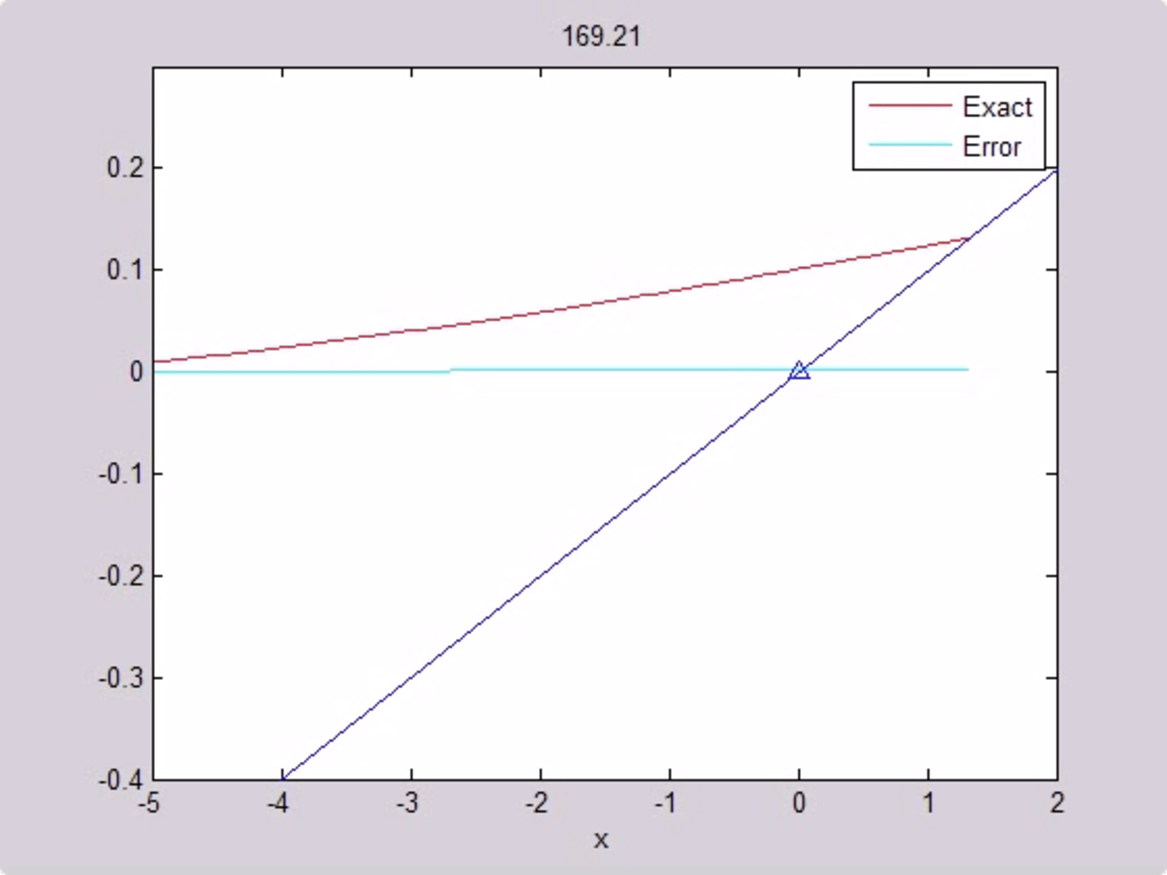
\includegraphics[width=.9\linewidth]{exactpara.pdf}}]{.9\linewidth}{}{exactpara.mov}
		\end{center}
	\end{frame}

	\begin{frame}
		\frametitle{Parabolic Case: Variable System Comparison}
		\begin{center}
		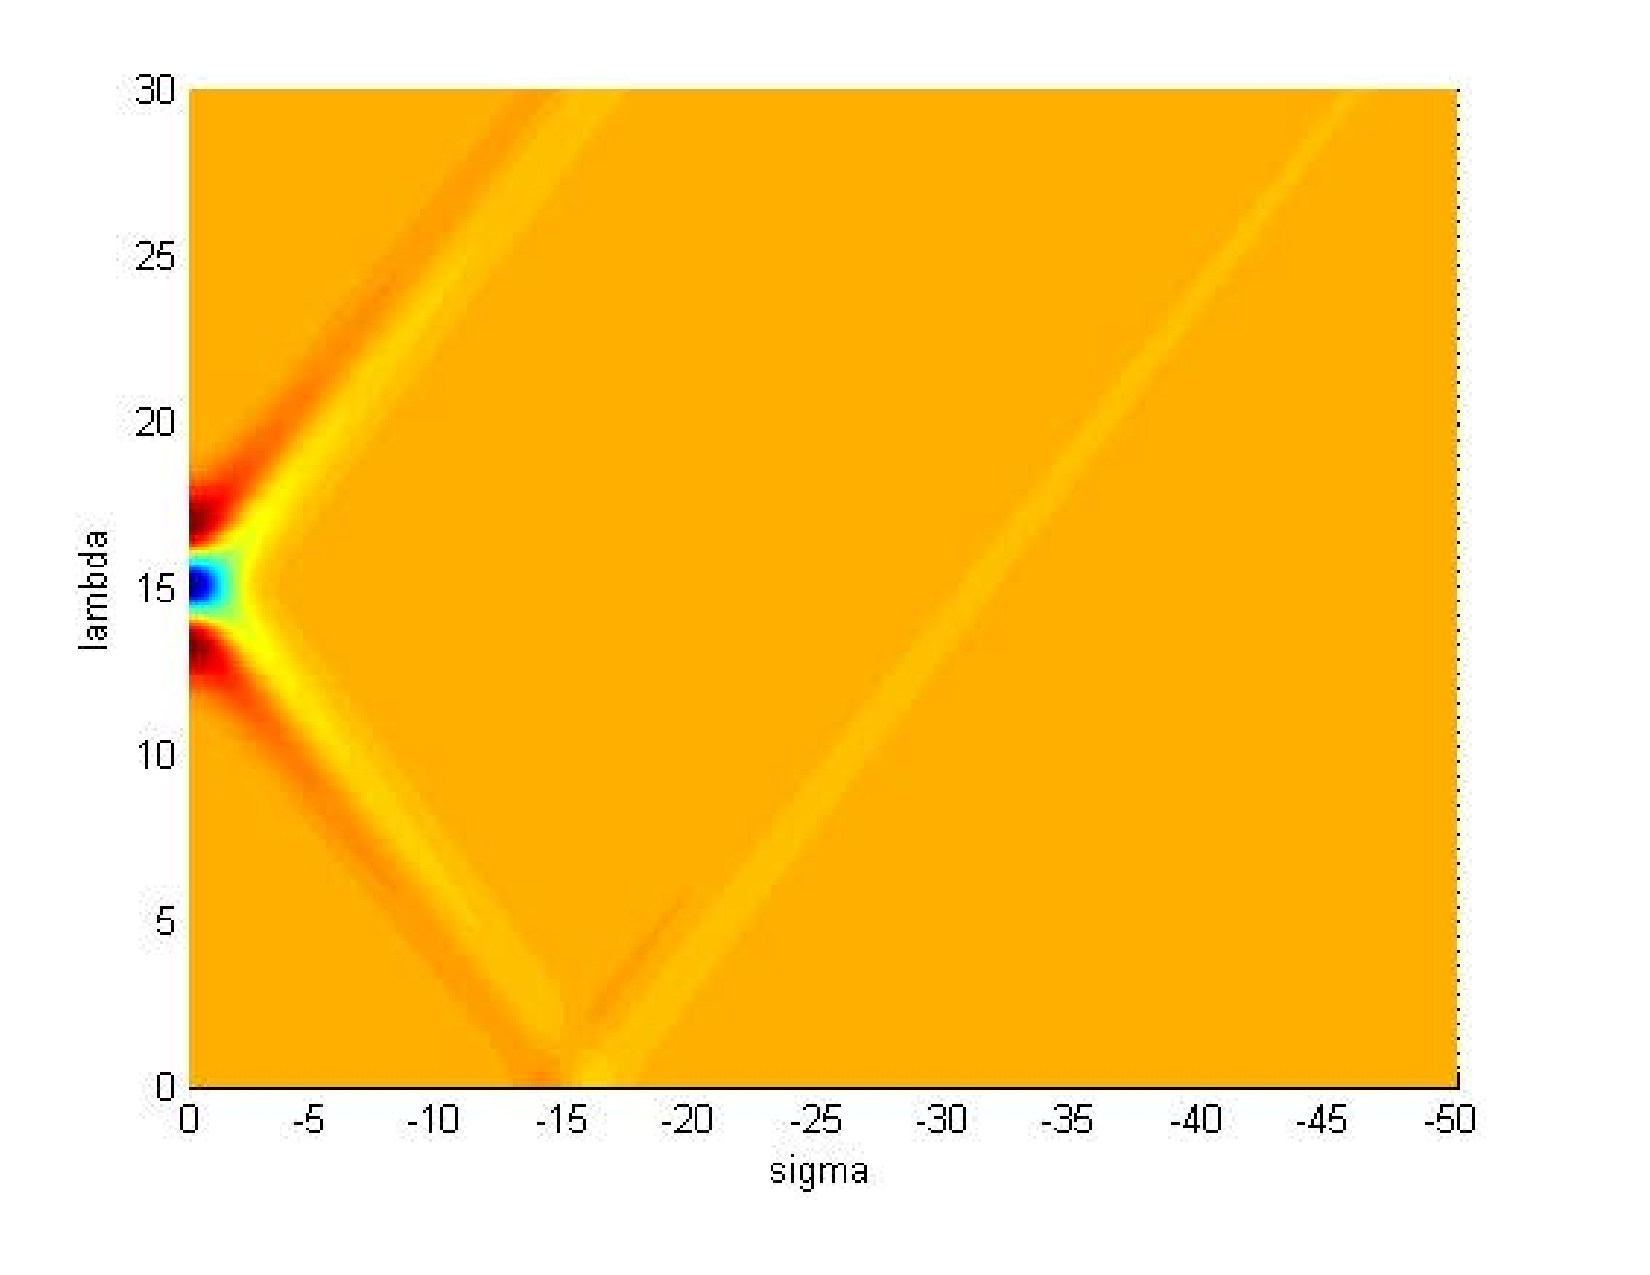
\includegraphics[width=0.5\textwidth]{NonPhys.pdf}
		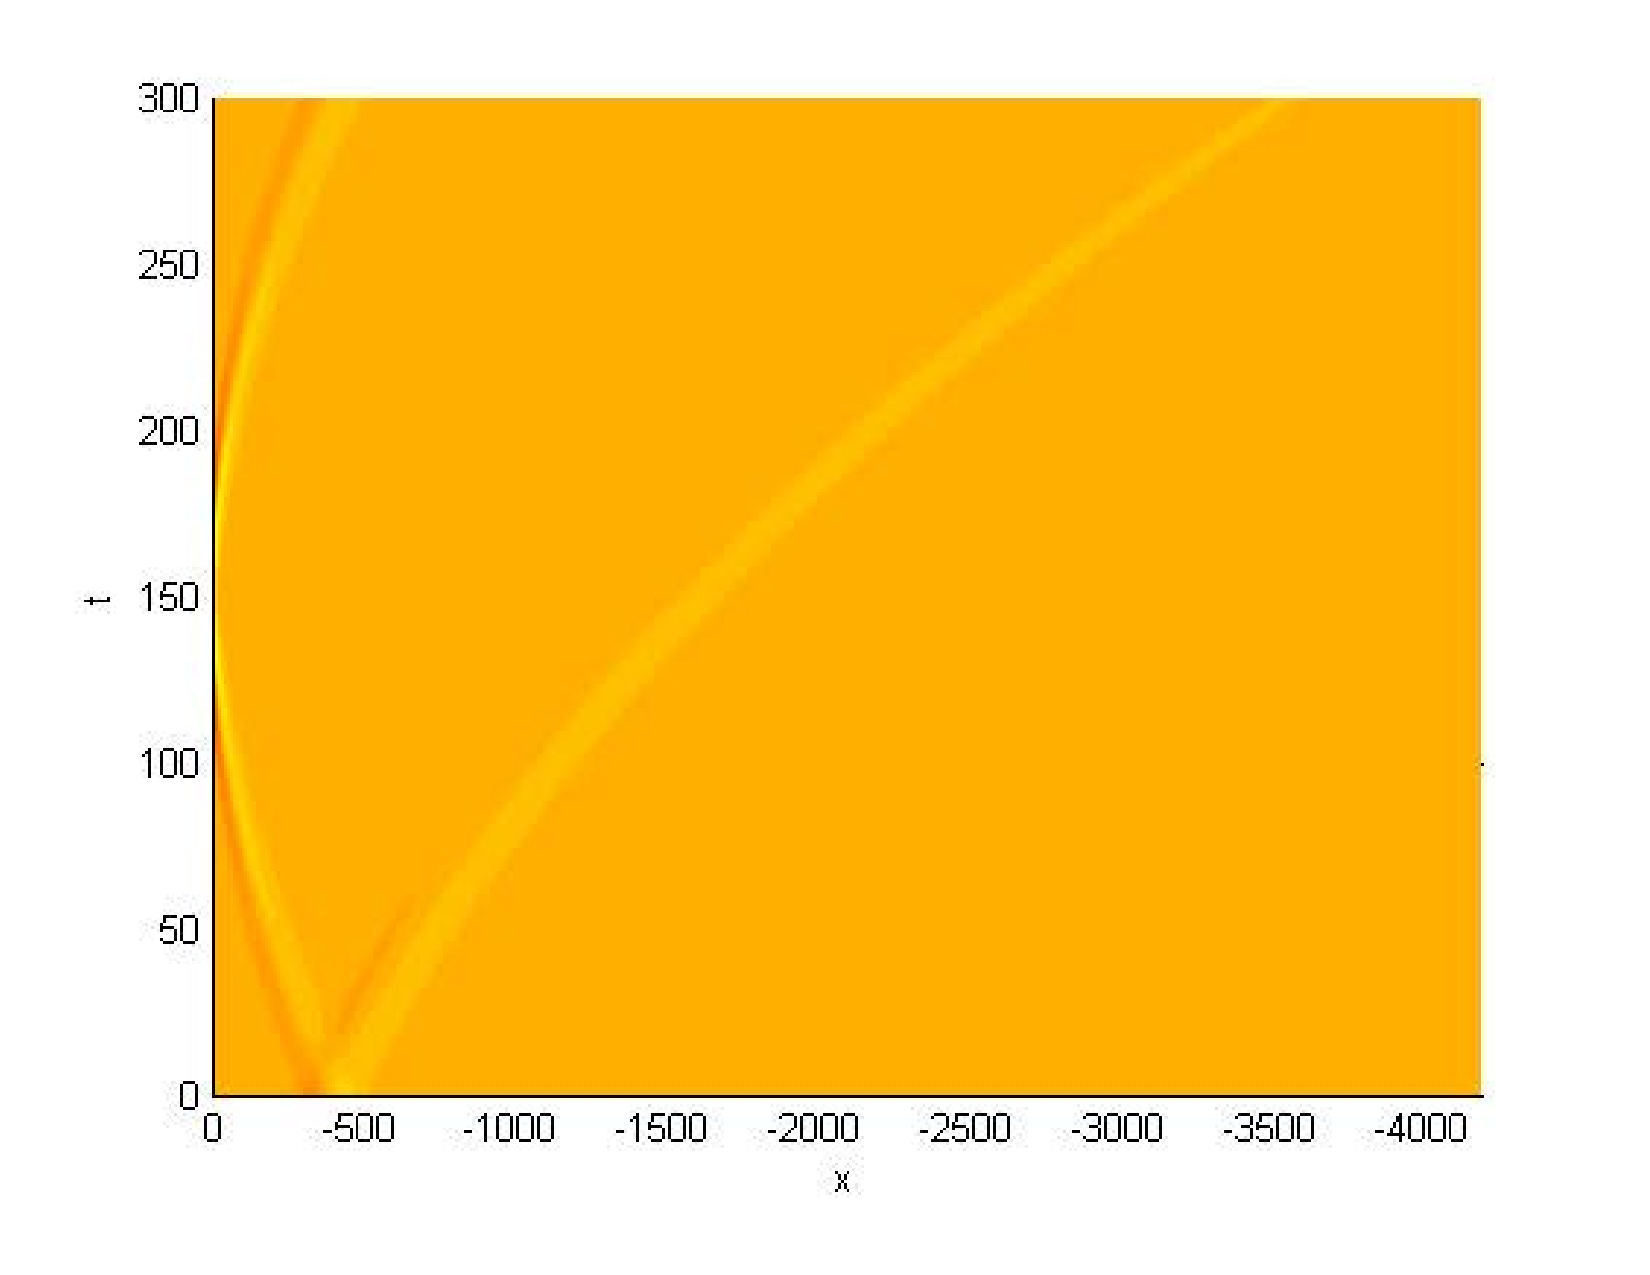
\includegraphics[width=0.5\textwidth]{Phys.pdf}
		\end{center}
		Left: N-Wave behavior in $\sigma, \lambda$.  Right: N-wave behavior in $x, t$.
		
		
	\end{frame}

	\begin{frame}
		\frametitle{Trapezoidal Case: in $\sigma$}
		\begin{center}
			\includemovie[text={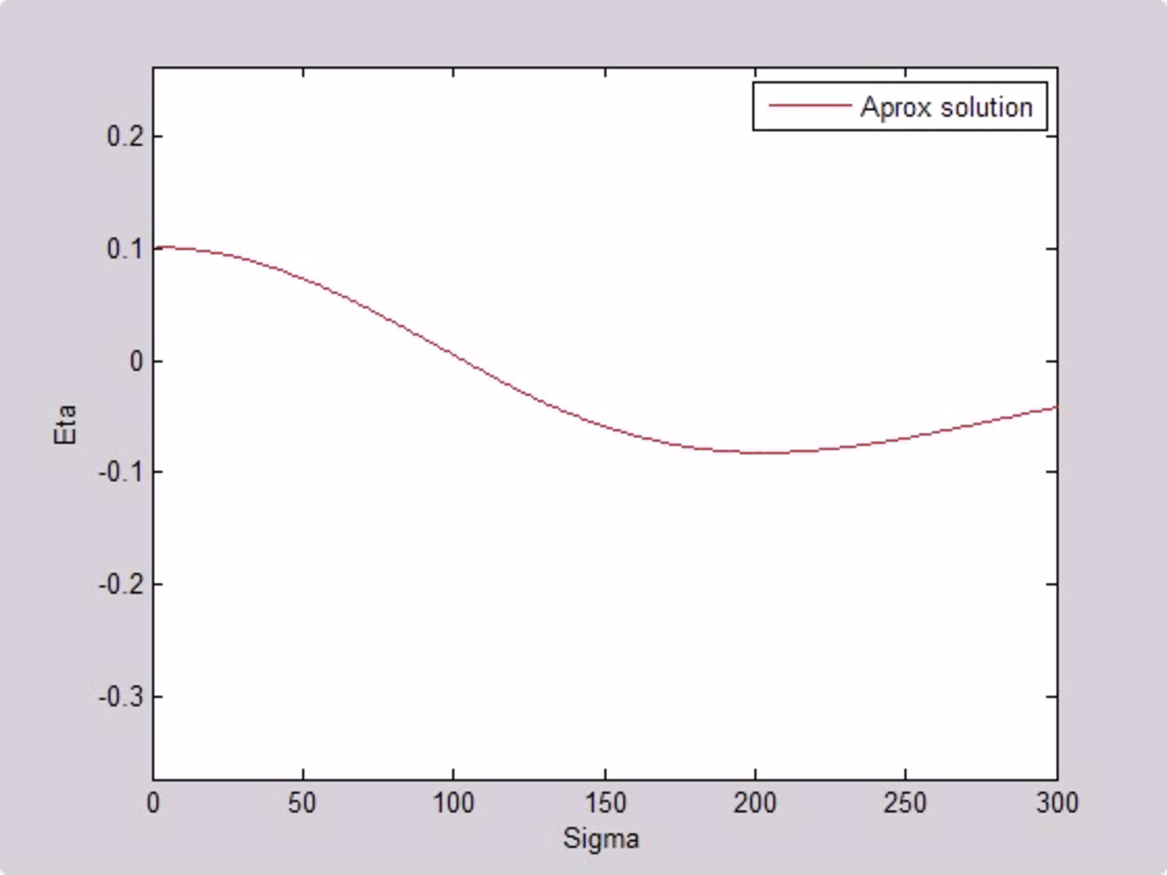
\includegraphics[width=.9\linewidth]{trapsigma.pdf}}]{.9\linewidth}{}{trapsigma.mov}
		\end{center}
	\end{frame}
	
	\begin{frame}
		\frametitle{Trapezoidal Case: in $x$}
		\begin{center}
			\includemovie[poster,text={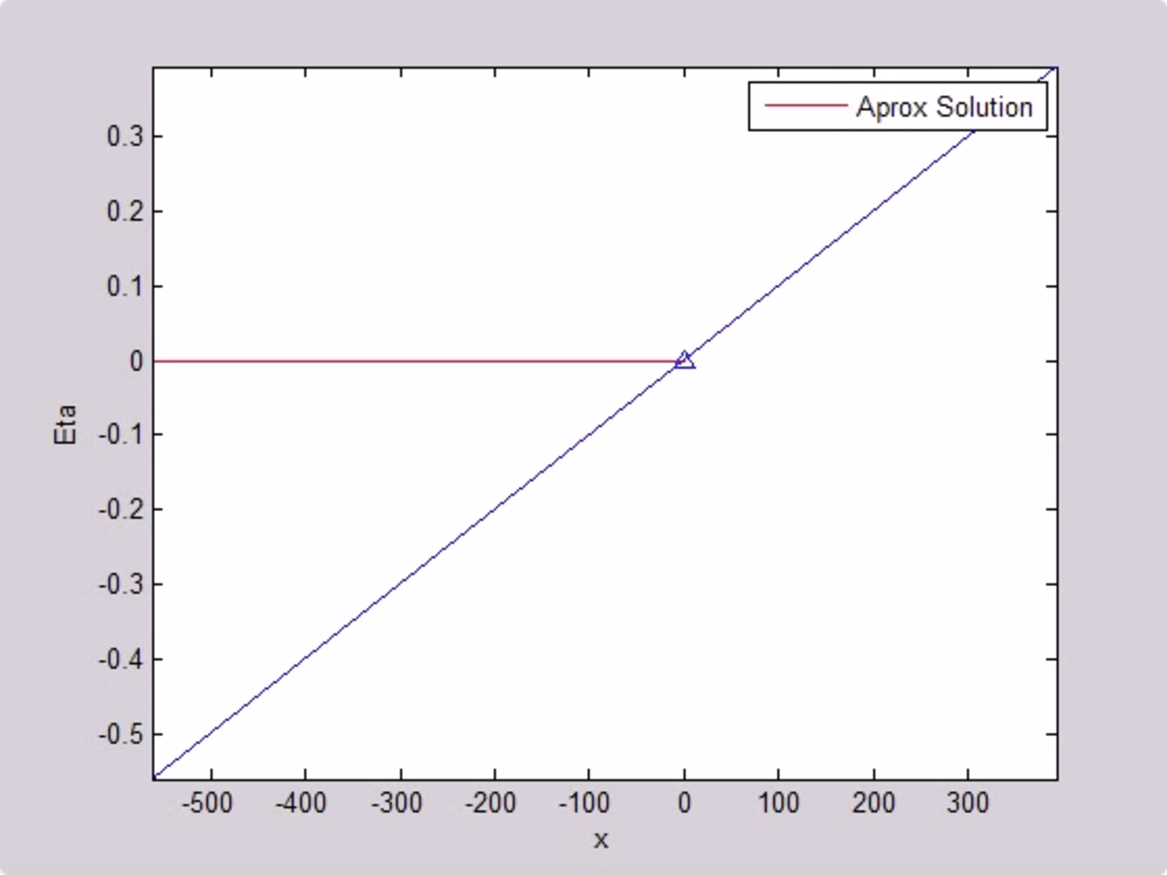
\includegraphics[width=.9\linewidth]{trapx.pdf}}]{.9\linewidth}{}{trapx.mov}
		\end{center}
	\end{frame}